\documentclass[conference]{IEEEtran}
\IEEEoverridecommandlockouts
% The preceding line is only needed to identify funding in the first footnote. If that is unneeded, please comment it out.
\usepackage{cite}
\usepackage{amsmath,amssymb,amsfonts}
\usepackage{algorithmic}
\usepackage{graphicx}
\usepackage{textcomp}
\usepackage{xcolor}
\usepackage{array}
\def\BibTeX{{\rm B\kern-.05em{\sc i\kern-.025em b}\kern-.08em
    T\kern-.1667em\lower.7ex\hbox{E}\kern-.125emX}}
\begin{document}

\title{Explainable Artificial Intelligence \\ {Methodology for Handwritten Applications}}

\author{\IEEEauthorblockN{Paul Whitten, Francis Wolff, Chris Papachristou}
\IEEEauthorblockA{\textit{Electrical, Computer, and Systems Engineering} \\
\textit{Case School of Engineering} \\
\textit{Case Western Reserve University} \\
Cleveland, OH, USA \\
pcw@case.edu, fxw12@case.edu, cap2@case.edu}

}

\maketitle

\begin{abstract}
There has been explosive growth of practical AI in recent years.
However, results of AI systems are not readily explainable to humans.
A major concern of current AI systems is an inability to explain decisions.
Explainable artificial intelligence has been posed to mitigate these concerns.
This work is an attempt to explore a methodology that provides explanations
for classification decisions.
\end{abstract}

\begin{IEEEkeywords}
explainable, artificial intelligence, machine learning
\end{IEEEkeywords}

\section{Summary}

Recent advances in Machine Learning (ML) have brought about wide adoption of ML algorithms for many applications.  Despite various successes, there is a reluctance to adopt ML in some applications because ML behaves like a black box, decision making by the black box is often not explainable to humans.  

This work approaches the widely studied problem of classifying images of handwritten digits into the ten decimal digit classes, zero through nine, from an Explainable Artificial Intelligence (XAI) perspective.

While we approach XAI for a specific classification problem in the MNIST handwritten digit database, which consists of 28x28 images of handwritten digits into the ten decimal digits, we feel the methodology translates to other problems of explainable classification among a finite set of classes.

This work aims to pose a means of explaining the classification to a human.  We do not wish to compete with established algorithms that perform exceptionally well in classification of input.   The effort required in applying the methodology in this work is significant compared to training a classifier that will act as a black box, and therefore not be explainable.

Our methodology for explainability is summarized as the use of explainable properties and related transformations of the input to make distinct classification decisions for each property.  Those distinct classifications are input to a voter to provide the best classification result.  Rationale, based on the explainable properties, are combined with the voter result to provide an explanation. 

The methodology is depicted in Fig.~\ref{voting} where $I_i$ represents the $i$th input.  The $P_x$ squares represent logic including distinct neural network architectures to make classifications based on properties where $x$ is 1 through n.  The Voter Model Engine is then used to consider each of the choices from the properties and provide the best decision.  Based on property results an explanation is assembled in XAI.   The explanation consists of the explainable properties that contribute to the classification.   The decision along with the property-based explanation is presented to a user.

 \begin{figure}[htbp]
\centerline{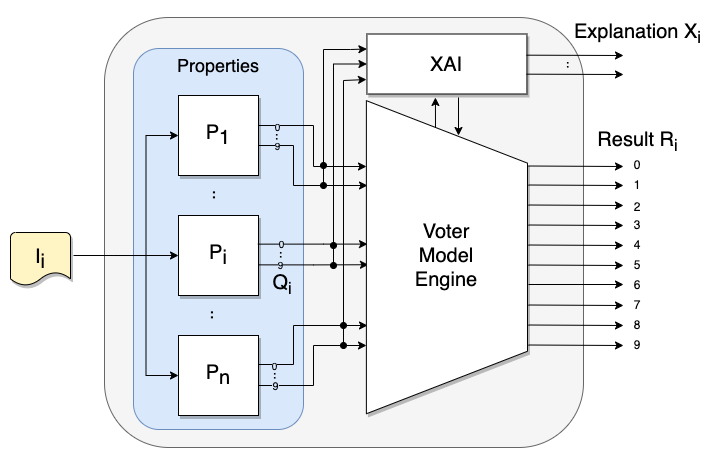
\includegraphics[width=95mm]{./images/voting_prop_nn_2.png}}
\caption{XAI Architecture Summary}
\label{voting}
\end{figure}

Further detailing explainable properties, we considered how explainable properties could be mapped to the input.  In this work we pose the use of input transformations that are related to explainable properties to aid in classification while providing human understandable rationale for classification decisions.  We chose to use one transformation per property in this work.  However, each property may have multiple such transformations.  This is represented in Fig.~\ref{proptrans} where the outer square represents the $j$th property square in Fig.~\ref{voting}.  The boxes labeled $T_x$ indicate the $x$th transformation of the input related to that property.  The transformed input is fed to a Neural Network Architecture (NNA) to make classification decisions based on the transformed input.  Output from the property transform decisions then flow to the voter as shown in Fig.~\ref{voting}.

 \begin{figure}[htbp]
\centerline{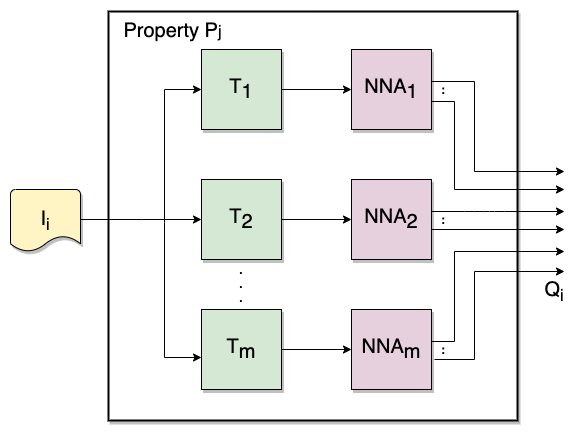
\includegraphics[width=90mm]{./images/property_transforms.png}}
\caption{Architecture of a single property for multiple tranformations.}
\label{proptrans}
\end{figure}

This work explores two voting model schemes.  Some voting schemes involve probabilistic algorithms while others involve ML algorithms.  Regardless of the voting algorithm, it was useful to construct and utilize a knowledgebase for storing detailed training and test results of the transformation NNs.  The knowledgebase was also important in estimating confidence used in voting algorithms. 
 
Our methodology for explainability involves the following steps:
\begin{itemize}
\item Discover explainable properties.
\item Define transformations for explainable properties.
\item Transform training data.
\item Produce trained explainable property-specific NNAs.
\item Build a Knowledgebase across the explainable properties.
\item Devise a voting scheme.
\item Use a test dataset to provide feedback.
\end{itemize}

The initial step is to discover explainable properties.  An explainable property is an attribute of a sample in the problem domain that may differentiate classes and provide a rationale for classification.  In the MNIST handwritten digit database, we pose explainable properties such as the stroke, circle, ellipse, lines, endpoints, and crossings.

\bgroup
\renewcommand{\arraystretch}{2}
%\setlength\tabcolsep{2mm}
\begin{figure}
\centering
\begin{tabular}{ | p{0.25\linewidth} | p{0.25\linewidth} | c c c | }
\hline
Property & Transform & $I_i$ &  &  $T_i$ \\
\hline \hline
Stroke & Skeleton & \raisebox{-.5\height}{
\includegraphics[width=10mm]{./digit-images/4-11.png}} & $\rightarrow$ & \raisebox{-.5\height}{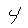
\includegraphics[width=10mm]{./digit-images/4-11-skel.png}} \\
\hline
Circle & Hough Circle & \raisebox{-.5\height}{
\includegraphics[width=10mm]{./digit-images/6-17.png}} & $\rightarrow$ & \raisebox{-.5\height}{
\includegraphics[width=10mm]{./digit-images/6-17-circle.png}} \\
\hline
Ellipse & Hough Ellipse & \raisebox{-.5\height}{
\includegraphics[width=10mm]{./digit-images/0-3.png}} & $\rightarrow$ & \raisebox{-.5\height}{
\includegraphics[width=10mm]{./digit-images/0-3-ellipse.png}} \\
\hline
Multiple Circle or Ellipse & Hough Ellipse and Circle & \raisebox{-.5\height}{
\includegraphics[width=10mm]{./digit-images/8-4.png}} & $\rightarrow$ & \raisebox{-.5\height}{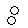
\includegraphics[width=10mm]{./digit-images/8-4-ellipse-circle.png}} \\
\hline
Enclosed Region & Flood Fill & \raisebox{-.5\height}{
\includegraphics[width=10mm]{./digit-images/0-2.png}} & $\rightarrow$ & \raisebox{-.5\height}{
\includegraphics[width=10mm]{./digit-images/0-2-fill.png}} \\
\hline
Enclosed Stroke & Skeleton Flood Fill & \raisebox{-.5\height}{
\includegraphics[width=10mm]{./digit-images/8-3.png}} & $\rightarrow$ & \raisebox{-.5\height}{
\includegraphics[width=10mm]{./digit-images/8-3-skel-fill.png}} \\
\hline
Crossings & Crossings & \raisebox{-.5\height}{
\includegraphics[width=10mm]{./digit-images/4-2.png}} & $\rightarrow$ & \raisebox{-.5\height}{
\includegraphics[width=10mm]{./digit-images/4-2-crossing.png}} \\
\hline
Endpoints & Endpoints & \raisebox{-.5\height}{
\includegraphics[width=10mm]{./digit-images/2-2.png}} & $\rightarrow$ & \raisebox{-.5\height}{
\includegraphics[width=10mm]{./digit-images/2-2-endpoint.png}} \\
\hline
Line & Hough Line & \raisebox{-.5\height}{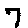
\includegraphics[width=10mm]{./digit-images/7-20.png}} & $\rightarrow$ & \raisebox{-.5\height}{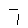
\includegraphics[width=10mm]{./digit-images/7-20-line.png}} \\
\hline
\end{tabular}
\centering
\caption{Sample Handwritten Digits ($I_i$) and Transforms ($T_i$)}
\label{transsample}
\end{figure}
\egroup

Data transformations are next defined and implemented to represent a sample for classification according to the initial step's explainable properties.  Transforms may be known algorithms of feature detection and extraction that represent property characteristics.  In our example, we used digital image processing techniques related to the properties.  Examples of original digit images and transforms are shown in Fig.~\ref{transsample}.  The stroke property used a morphological skeleton transformation.  A Hough transform was used with the appropriate formula for circle and ellipse properties.  The line property utilized the skeleton and a linear Hough Transform to identify lines over a threshold of six pixels.  The Multiple circle or ellipse used circle and ellipse transforms with non-overlapping results.  The morphological skeleton was also used to find endpoints, pixels with only one activated neighbor, and crossings, pixels with more than two activated neighbors.   The endpoints and crossings are shown with neighboring pixels partially activated to aid in ML classification.
 
We next generate a transformed training dataset by submitting all elements from the original training set to the property transformations.  The output from each property transformation is stored separately for training each property-specific NNA. 

The next step involves initializing unique NNAs representing each property and then using supervised ML techniques to train the NNAs using only the output of that particular property transform and the original labels.  This results in trained NNAs for each property.

After training, we again process the training set and populate a knowledgebase.  The knowledgebase stores the original training label, and each property's classification results from the property NNA.  The knowledgebase is used in constructing the voting strategy. 

We next devise a voting strategy using information from the knowledgebase.  The purpose for the voting strategy is to select among the multiple and potentially conflicting votes from the properties.

The first voting scheme we present is probabilistic.  In this scheme, we use the knowledgebase to identify each NNA's likelihood to correctly digits.  Likelihoods are weighted and compared against the alternative classifications to provide confidence metrics for classification.  If there is disagreement among properties, this scheme will produce multiple classifications each with a confidence metrics.  The classification with the highest confidence is selected by the voter.

The second classification scheme utilizes the knowledgebase as a set to train a NNA to select a digit on property transform results.  Using this scheme, we show very good results.  In this scheme we do not produce a confidence metric from the Knowledgebase but can present each digit's value form the voting NNA as confidence.

Finally, when test data is presented to the XAI architecture, we evaluate the results and determine if they are sufficient or if more properties are needed.

Results obtained using the MNIST digit database using the probabilistic voting engine were $91.8\%$ while results obtained from the NN voting engine were $97.3\%$ using the MNIST test dataset.

The 9 properties we identified along with transformation and identifiers for those properties, used in as shown in TABLE ~\ref{table:tblproptrans}.

The Stroke property is meant to minimally represent the digit, removing the variability of the line thickness in among digits.  Using the skeleton, which is a one pixel connected representation preserving the topology of the digit.  We utilized the Lee\cite{Lee1994} algorithm for obtaining skeletons of the MNIST handwritten digits.

Mean digit intensity plots of the property transformation NNAs are shown for training data for digits 5 and 6 in the following figures.

Results obtained using the probabilistic voting engine were $91.8\%$ while results obtained from the NN voting engine were $97.3\%$ using the MNIST test dataset.

\begin{table}
\caption{Properties, Transforms and Property Identifiers}
\centering
\begin{tabular}{| c | c | c |}
\hline
 Explainable Property & Transform(s) & Identifier \\
\hline\hline
Stroke & Skeleton & $P_0$ \\
\hline
Circle & Hough Circle & $P_1$ \\
\hline
Crossings & Crossing Point & $P_2$ \\
\hline
Ellipse & Hough Ellipse & $P_3$ \\
\hline
Ellipse + Circle & Hough Ellipse and Circle & $P_4$ \\
\hline
Endpoints & Endpoints & $P_5$ \\
\hline
Enclosed Region & Flood Fill & $P_6$ \\
\hline
Line & Hough Line & $P_7$ \\
\hline
Enclosed Region of Skeleton & Skeleton Flood Fill & $P_8$ \\
\hline
\end{tabular}
\label{table:tblproptrans}
\end{table}

\begin{table*}
\caption{Digit 5 Outputs}
\centering
\begin{tabular}{ | c ||  c | c | c | c | c | c | c | c | c |}
 digit 5 & $P_0$ & $P_1$ & $P_2$ & $P_3$ & $P_4$ & $P_5$ & $P_6$ & $P_7$ & $P_8$ \\
\hline \hline
pct. correct  & 100.0 & 14.2 & 5.7 & 20.8 & 21.5 & 85.4 & 3.8 & 70.0 & 5.5 \\
\hline
$\sigma$ & 0.300& 0.076& 0.082& 0.068& 0.089& 0.252& 0.074& 0.211& 0.077 \\
\hline
k & 10.000& 3.995& -1.864& 5.555& 6.229& 9.550& -1.941& 9.779& -2.063 \\
\hline
skew & 3.162& 1.913& 0.330& 2.324& 2.413& 3.073& -0.025& 3.116& 0.061 \\
\hline
0 & 0.000 & 0.115 & 0.208 & 0.093 & 0.073 & 0.002 & 0.007 & 0.023 & 0.020 \\
\hline
1 & 0.000 & 0.048 & 0.223 & 0.057 & 0.044 & 0.111 & 0.193 & 0.008 & 0.183 \\
\hline
2 & 0.000 & 0.048 & 0.051 & 0.058 & 0.053 & 0.001 & 0.089 & 0.027 & 0.069 \\
\hline
3 & 0.000 & 0.162 & 0.082 & 0.154 & 0.154 & 0.002 & 0.149 & 0.079 & 0.178 \\
\hline
4 & 0.000 & 0.046 & 0.006 & 0.056 & 0.045 & 0.003 & 0.122 & 0.019 & 0.130 \\
\hline
5 & 1.000 & 0.300 & 0.200 & 0.284 & 0.345 & 0.849 & 0.186 & 0.732 & 0.185 \\
\hline
6 & 0.000 & 0.097 & 0.069 & 0.059 & 0.090 & 0.009 & 0.027 & 0.036 & 0.037 \\
\hline
7 & 0.000 & 0.045 & 0.167 & 0.067 & 0.041 & 0.001 & 0.185 & 0.011 & 0.212 \\
\hline
8 & 0.000 & 0.109 & 0.022 & 0.094 & 0.101 & 0.014 & 0.005 & 0.042 & 0.005 \\
\hline
9 & 0.000 & 0.044 & 0.019 & 0.069 & 0.043 & 0.009 & 0.032 & 0.034 & 0.028 \\
\hline
false pos rt & 0.0 & 0.5 & 0.2 & 0.4 & 0.7 & 0.4 & 0.0 & 0.3 & 0.0 \\
\hline
false neg rt & 0.0 & 84.8 & 94.1 & 78.8 & 78.3 & 13.4 & 96.2 & 29.2 & 94.5 \\
\hline
\end{tabular}
\end{table*}



\begin{table*}
\caption{Digit 6 outputs}
\centering
\begin{tabular}{ | c ||  c | c | c | c | c | c | c | c | c |}
 digit 6 & $P_0$ & $P_1$ & $P_2$ & $P_3$ & $P_4$ & $P_5$ & $P_6$ & $P_7$ & $P_8$ \\
\hline \hline
pct. correct  & 100.0 & 46.5 & 49.5 & 32.0 & 49.0 & 93.3 & 81.8 & 70.7 & 83.2 \\
\hline
$\sigma$ & 0.300& 0.112& 0.130& 0.094& 0.133& 0.264& 0.240& 0.209& 0.246 \\
\hline
k & 10.000& 8.507& 8.617& 9.864& 9.469& 9.955& 9.935& 9.889& 9.930 \\
\hline
skew & 3.162& 2.842& 2.886& 3.132& 3.048& 3.153& 3.148& 3.138& 3.147 \\
\hline
0 & 0.000 & 0.100 & 0.042 & 0.069 & 0.080 & 0.020 & 0.001 & 0.034 & 0.004 \\
\hline
1 & 0.000 & 0.052 & 0.050 & 0.066 & 0.048 & 0.005 & 0.035 & 0.011 & 0.033 \\
\hline
2 & 0.000 & 0.057 & 0.135 & 0.064 & 0.061 & 0.020 & 0.022 & 0.028 & 0.013 \\
\hline
3 & 0.000 & 0.095 & 0.046 & 0.070 & 0.079 & 0.002 & 0.027 & 0.051 & 0.032 \\
\hline
4 & 0.000 & 0.039 & 0.044 & 0.067 & 0.040 & 0.000 & 0.027 & 0.046 & 0.023 \\
\hline
5 & 0.000 & 0.101 & 0.065 & 0.052 & 0.086 & 0.008 & 0.028 & 0.029 & 0.024 \\
\hline
6 & 1.000 & 0.426 & 0.482 & 0.380 & 0.495 & 0.890 & 0.818 & 0.725 & 0.837 \\
\hline
7 & 0.000 & 0.057 & 0.049 & 0.077 & 0.047 & 0.000 & 0.033 & 0.007 & 0.038 \\
\hline
8 & 0.000 & 0.027 & 0.086 & 0.068 & 0.030 & 0.034 & 0.004 & 0.041 & 0.001 \\
\hline
9 & 0.000 & 0.029 & 0.026 & 0.077 & 0.038 & 0.000 & 0.007 & 0.027 & 0.005 \\
\hline
false pos rt & 0.0 & 2.6 & 2.5 & 0.5 & 2.2 & 0.7 & 0.2 & 0.6 & 0.0 \\
\hline
false neg rt & 0.0 & 53.3 & 50.1 & 67.5 & 50.7 & 6.6 & 18.1 & 28.1 & 16.8 \\
\hline
\end{tabular}
\end{table*}



\begin{figure*}[htbp]
\centerline{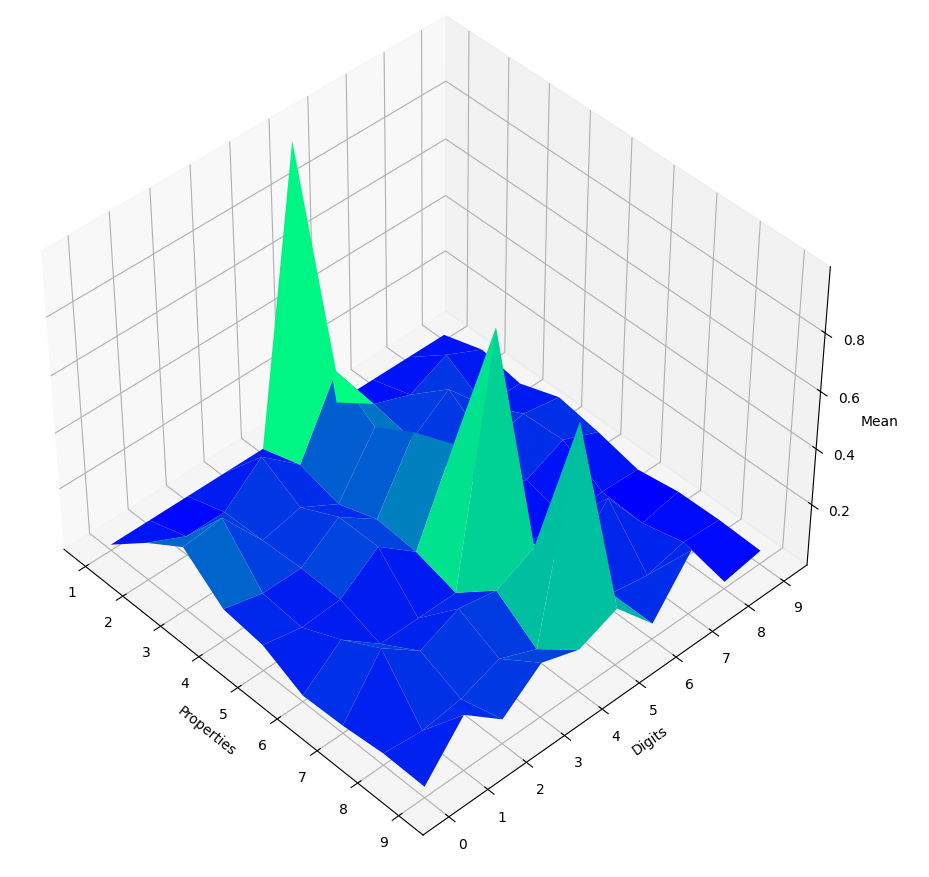
\includegraphics[width=160mm]{./images/digit-5.png}}
\caption{Property Transformation votes for the digit 5}
\label{digit5votes}
\end{figure*}

\begin{figure*}[htbp]
\centerline{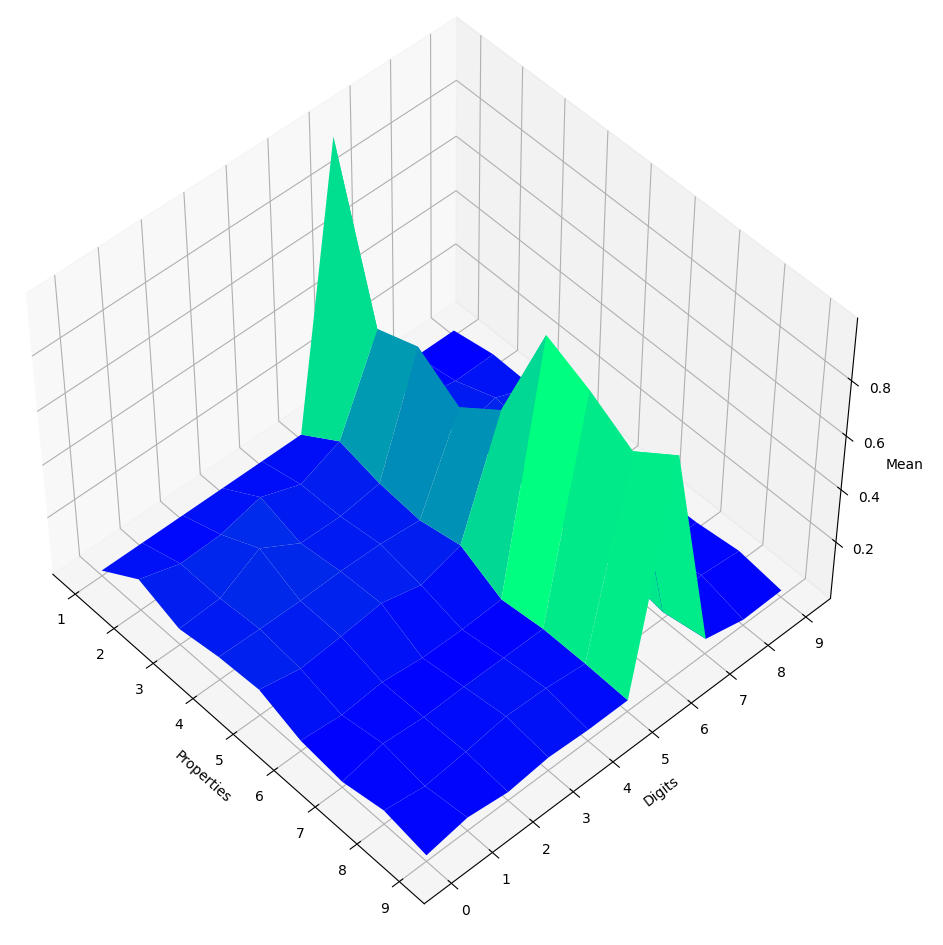
\includegraphics[width=160mm]{./images/digit-6.png}}
\caption{Property Transformation votes for the digit 6}
\label{digit6votes}
\end{figure*}


\section{References}
\bibliographystyle{plain}
\bibliography{references}{}


\end{document}
